\subsection{Into}
Bei der Funkverbindung wurde auf das Radiohead-Paket\cite{rh} zurückgegriffen. Dieses Paket unterstützt viele gängige Sender/Empfänger-Kombinationen. Des weiteren ist anzumerken das hier die \grqq einfache\grqq  ASK\footnote{Amplitude Shift Keying/Amplitudenumtastung} Modulationsart verwendet wird. Dies wird durch das sogenannte On-Off Keying realisiert. \newline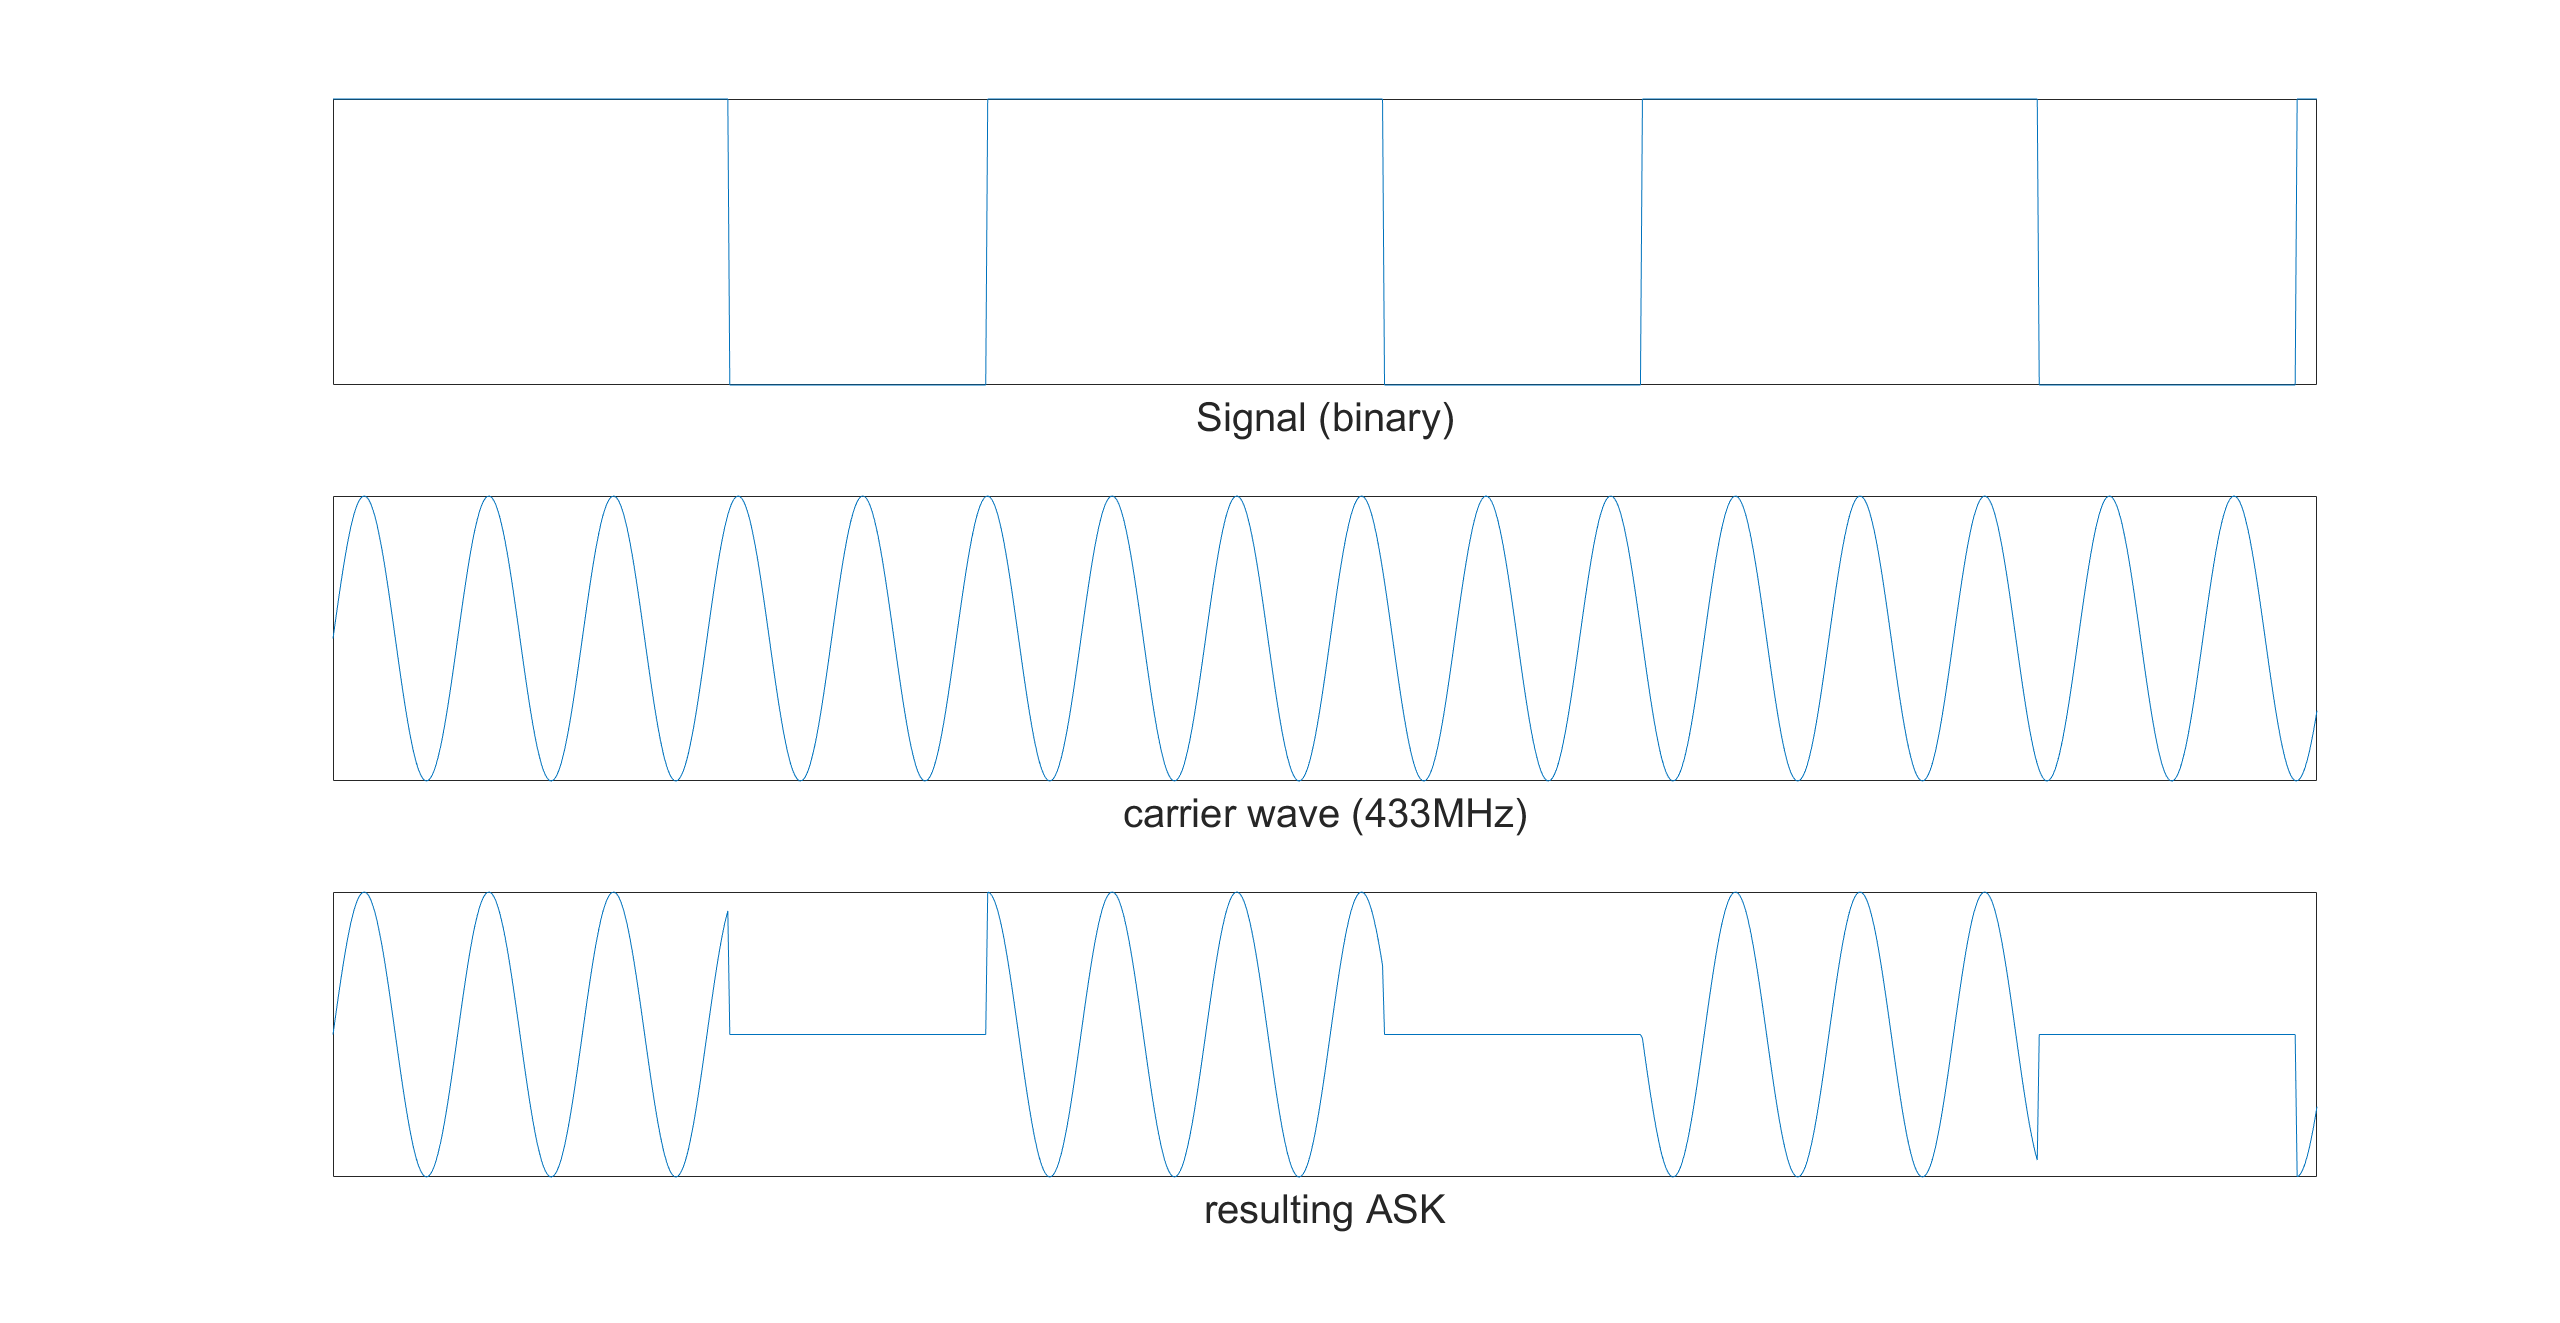
\includegraphics[width=\textwidth]{Hauptteil/sw/intro/ask.png}